\documentclass[12pt,fleqn]{article}\usepackage{../../common}
\begin{document}
Zaman Serileri 

Bir zaman serisi $t$ anında belli bir değeri olan veri noktalarıdır. Finans
bağlamında çoğunlukla birbirini takip eden iki veri noktası arasında bağlantı
olduğu ispatlanmıştır. Altta örnek bir zaman serisi görüyoruz; 500 senetin
ağırlıklı ortalaması olan S\&P 500 indisinin zaman göre gidişatı (düzeltilmiş
kapanış hesaplarını baz alarak),

\begin{minted}[fontsize=\footnotesize]{python}
import pandas as pd
df = pd.read_csv('../tser_risk/SPY2.csv',parse_dates=True,index_col='Date')
df = df.sort_index()
df = df[df.index > '1950-01-01']
\end{minted}

\begin{minted}[fontsize=\footnotesize]{python}
df['Adj Close'].plot()
plt.savefig('tser_intro_01.png')
\end{minted}

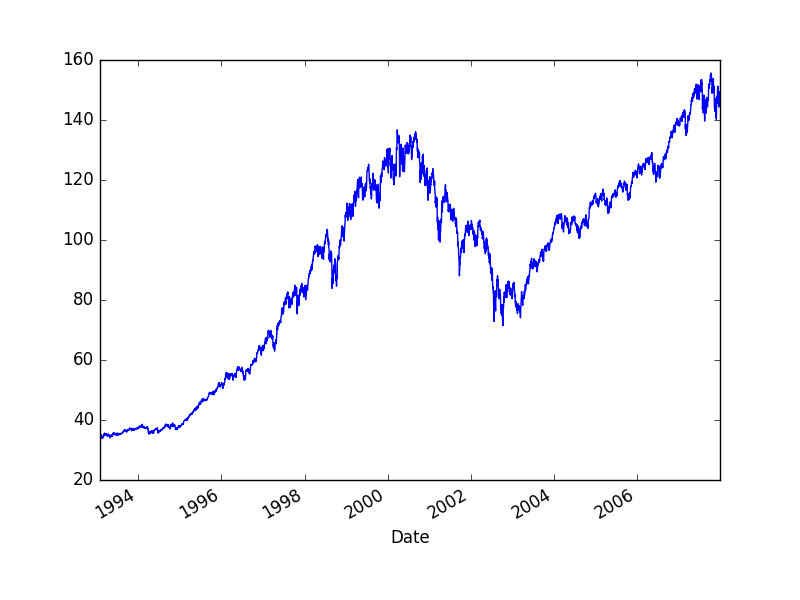
\includegraphics[height=6cm]{tser_intro_01.png}

Zaman serileri hakkında önemli bir bilgi onların ``getirisidir
(returns)''. Getiri hesabı $t$ ile $t-1$ arasındaki değişim oranı, yani
$X_{t}-X_{t-1}/X_{t-1}$. Bu sayıyı 100 ile çarpınca ise yüzde değişimi elde
ederiz. Pandas ile,

\begin{minted}[fontsize=\footnotesize]{python}
returns = df['Adj Close'].pct_change()
print returns.head()
\end{minted}

\begin{verbatim}
Date
1993-01-29         NaN
1993-02-01    0.007022
1993-02-02    0.002034
1993-02-03    0.010728
1993-02-04    0.004303
Name: Adj Close, dtype: float64
\end{verbatim}

İlk veri noktası \verb!NaN! oldu çünkü bir önceki veri noktası yok.

Bu değişim oranı getiri zaman serilerinin doğasına göre bir yukarı bir aşağı
iner, çünkü arz talebe, ya da diğer sebeplere göre senet fiyatları bazen çıkar,
bazen düşer. Bir trend de olabilir tabii, bazen daha çok çıkabilir, bazen daha
çok inebilir. Tamama bakılınca ve bu {\em getirilerin}, dikkat fiyat veri
noktalarının değil, frekansını düşünürsek bu getirilerin bir dağılımdan geldiği
kabul edilebilir, histograma bakalım,

\begin{minted}[fontsize=\footnotesize]{python}
returns.plot(kind='hist',bins=100)
plt.savefig('tser_intro_02.png')
\end{minted}

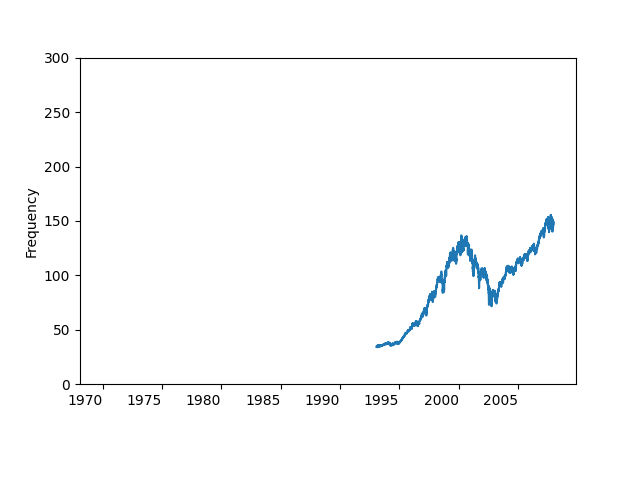
\includegraphics[height=6cm]{tser_intro_02.png}

İstatistikten hatırlarsak histogram bize belli değerlerin hangi frekansla
görüldüğünü söylüyor. Bir histogram ile bir olasılık dağılımı arasında yakın
bağlantılar var, histogram bir dağılımın sayısal hali denebilir. Şekil Gaussian
dağılımına benziyor. Fakat genel bağlamda finans serilerinde tüm getirilerin
Gaussian olduğunu direk söylemek hatalı olur, bu konuyu işleyeceğiz.

Histogramı okurken şöyle çıkarımlar yapabiliriz; mesela yüzdeliklere bakarız, ve
diyelim ki yüzde 5 noktasında (histogram alanının yüzde 5'ine tekabül eden
x-eksenindeki nokta) değeri okuruz, bu değer 0.02 civarında gibi duruyor; o
zaman varılacak sonuç şöyle seslendirilebilir, ``100 günün 5 gününde \%2'lik
düşüşler görülebilir''.  Bu mantıklı herhalde, çünkü bir dağılımdaki belli bir
alan o alanın x-eksenindeki değerlerin ortaya çıkma olasılığını verir. Ortaya
çıkma birimi gün ise, yüzde 5, 100 gün içinde 5 gün demektir.

Çıplak gözle bakmak yerine direk veriden bu hesabı yapabiliriz,

\begin{minted}[fontsize=\footnotesize]{python}
print returns.quantile(q=0.05)
\end{minted}

\begin{verbatim}
-0.0177541105196
\end{verbatim}

Gaussian durumu ilginç; kabaca Gaussian kabulü yapılabilir, fakat literatürdeki
çoğu yazı finans serilerinde düşüşlerin daha sert olduğunu belirtir, yani
Gaussian'da sola, negatif değerlere doğru bir yamukluk (skew) vardır. Ayrıca
fazla sayıda zaman serilerine bakıldığında her iki yönde aşırı değerlerin
Gaussian faraziyesine uymayan şekilde daha fazla olduğu tespit edilmiştir, yani
finans getirilerinin dağlımı ``etekleri kabarık'' bir Gaussian'dır, daha doğrusu
Öğrenci t dağılımıdır. Fakat basitleştirme amacıyla Gaussian kullanılabilir,
tabii bu faraziyenin sınırlarını bilmek şartıyla.

Oynaklık (Volatility)

Artışların, düşüşlerin ne kadar sert, yüksek boyutta olduğunun iyi bir
göstergesi olarak oynaklık kullanılır, oynaklık üstteki Gaussian faraziyesinden
hareketle getirilerin standart sapması $\sigma$'dan (sigma) ibarettir, o zaman
tanıdığımız, bildiğimiz $\sigma$ hesabı direk burada kullanılabilir,

\begin{minted}[fontsize=\footnotesize]{python}
print returns.std()
\end{minted}

\begin{verbatim}
0.010654265587
\end{verbatim}

Üstte en soldan yüzde 5 noktasına baktık, her iki yönde tek sigma büyüklüğünde
bir getirinin Gaussian bağlamında alanın yüzde 68'ine tekabül ettiğini
biliyoruz.

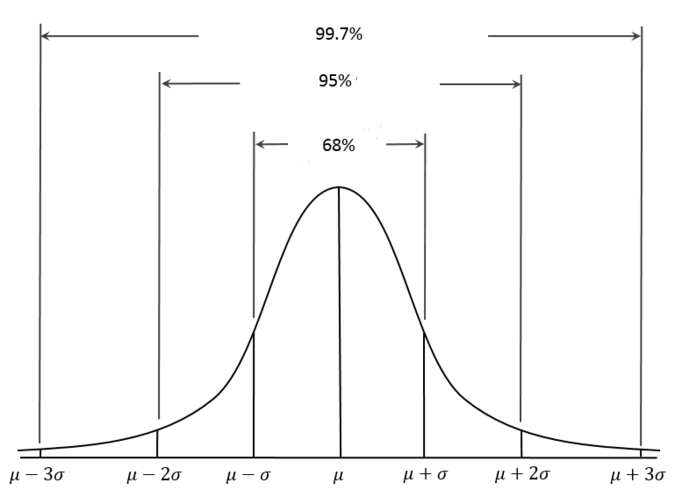
\includegraphics[height=6cm]{gausspercentiles.png}

Bu demektir ki getiriler Gaussian ile dağılmışsa artı ya da eksi tek sigmalık
(ya da ondan azı olan) değişimlerin olasılığı yüzde 68'dir. İki sigmalık (ve
daha azı) büyüklüğünde getirilerin olasılığı yüzde 95'tır.

Günlükten yıllığa geçmek için getiriler için direk 256 ile çarpılır, bir yıl
içinde aşağı yukarı 256 tane iş günü vardır. Standart sapma geçişi için
$\sqrt{256}$ yani 16 ile çarpmak gerekir. Bazıları 252 kullanıyor, çünkü NYSE
borsasında 252 günde alışveriş yapılabilir. Karekök basitliği sebebiyle bizce
256 daha uygun.

Niye $\sqrt{252}$ ile çarpıyoruz? Bu durum varlık fiyat zaman serisinin Brownian
yürüyüş olmasıyla alakalı. BM serilerinde varyans $t$ ile doğru orantılıdır,
yani başlangıç noktasından ne kadar uzaklaşırsak varyans o kadar büyür, çünkü
her adımdaki varyans toplanır (oynaklık standart sapmadır, ki bu varyansın
kareköku o sebeple zamanın kareköku ile çarpıyoruz). {\em Olasılıksal Calculus}
yazısında bu matematiği görüyoruz. Kabaca düşünmek gerekirse BM 'sarhoş
yürüyüşü' ise ve bu yürüyüş her adımda rasgele bir hareket yapıyorsa, bu adımlar
toplana toplana tabii ki başlangıç noktasından bizi çok uzak noktalara
taşıyabilir (ve geri getirebilir).

Kabaca borsacılar bilir ki senetlerin yıllık standart sapması \%20 civarıdır,
daha güvenli olan tahvillerin ise \%1.5. Kaldıraç, yani borç kullanıldığı zaman,
mesela 10 kat kaldıraç olduğunu düşünelim, bu oynaklığı 10 ile çarpmak
demektir. Normal bir hisse için 10 kat kaldıraç sizi yıllık sigma \%200'e
seviyesine getirir, bu günde \%200 / 16 = \%12.5 demektir. Eğer getirimiz son
derece iyimser bir bakışla yılda \%200 olsaydı, bu günlük \%0.8 olurdu (256 ile
böldük) ve ters yönde bir sigma'lık düşüş geldiği anda 0.8-12.5=-\%11.7'ı
görürdük, diğer yönde 0.8+12.5=\%13.3. Fakat bu demektir ki günlük getiriler 100
günün 68'inde -\%11.7 ile \%13.3 arasında gidip geliyor, 95'inde \%-24.2 ile
\%25.8 arasında gidip geliyor. O zaman günlerin 100-95=\%5'inde bu bantın her
iki taraftan dışında (en azdan daha az, en fazladan fazla) rakamlar göreceğiz
demektir, 5/2=\%2.5 kadar zamanda \%-24.2'dan daha fazla düşüş olacak demektir
bu! 100 günde 2.5 demek, 40/1 oran anlamına geliyor, bir ay içinde 20 işgünü
olduğuna göre bahsedilen olayın aşağı yukarı iki ayda bir ortaya çıkması
muhtemeldir. Yani iki ayda bir günde -\%24.2'lik getiri kaybı! Bu frekans olarak
çok ciddi bir kayıptır, ve psikolojik olarak yatırımcıyı rahatsız edecektir. Bu
noktaya nasıl geldiğimizi hatırlayalım, son derece iyimser bir getiri, 10 kat
seviyesinde bir kaldıraçla başlamıştık.

Sharpe Oranı (Sharpe Ratio)

Sharpe oranı (SO) bir işlem stratejisinin, ya da bir varlığı elde tutmanın, ki
basit olsa bile bu da bir strateji, ne kadar karlı olacağını ölçek bir
hesaptır. Hesaplamak için getirileri riske göre uyarlarız. Formel olarak
getirinin ortalamasını aynı periyottaki standart sapmaya böleriz. Bu bize günlük
SO verir, yıllığı hesaplamak için $\sqrt{256}$ ile çarpmak gerekir. 

Kayıpları Hesaplamak

Rasgele sayı üretimi kullanarak zaman serisi üretmek simülasyon amaçlı faydalı
bir işlem; mesela istediğimiz hedeflediğimiz oynaklık seviyesi, ve SO üzerinden
belli bir yamukluğa sahip bir zaman serisini üretip (daha doğrusu getirileri
üretip sonra zaman kumulatif hesap ile seriyi üretip), onun üzerinden muhtemel
kayıpların ne seviyede olacağını görebiliriz. Diyelim ki hiç yamukluğu olmayan,
yüzde 50 oynaklık hedefi ile yıllık SÖ=0.5 üzerinden kayıplar ne olacaktır?

\begin{minted}[fontsize=\footnotesize]{python}
from commonrandom import arbitrary_timeindex, skew_returns_annualised
from common import account_curve
import pandas as pd

want_skew = 0.0
annualSR = 0.5
days = 256*10. # 10 senelik
res = skew_returns_annualised(annualSR=annualSR, want_skew=want_skew, \
                              voltarget=0.50, size=days) 
df = pd.DataFrame(res)
df = df.set_index(pd.to_datetime(df.index, unit='d'))
df['cum'] = (1+df).cumprod() # kumulatif - zaman serisinin kendisi burada
\end{minted}

Her ayın en kötü günlük kaybı, 100,000 Eur'lik sermaye üzerinden diyelim,

\begin{minted}[fontsize=\footnotesize]{python}
K = 1000; capital = 100*K
print capital * df[0].quantile(q=0.05)
\end{minted}

\begin{verbatim}
-5144.01215594
\end{verbatim}

0.05 yüzdelik dilimine (quantile) baktık, çünkü 100 gün içinde 5 gün 20 gün
içinde 1 gün demektir, bir ayda 20 iş günü olduğunu kabul edersek her ayın en
kötü kaybını bu şekilde hesaplayabiliriz.

Yüzdelik dilime bakmak güzel bir numara; getirilerin dağılımına bakıyoruz, ama
yamukluk sebebiyle bu dağılımın analitik bir formülü elimizde yok, sadece
sayısal bir dağılım var, yani verinin kendisi. Bu sayısal dağılımda yüzdelik
dilime bakmak, analitik durumda ters kumulatif yoğunluk fonksiyonu (inverse cdf)
hesabı yapmak ile eşdeğerdir, yani ``olasılığı (olasılık yoğunluk alanı, ya da
cdf) vesaire olan şey hangi değere tekabül eder?'' sorusunun cevabını sayısal
olarak buluyoruz.

Her sene en kötü haftalık kayıp için elimizdeki günlük getirileri haftalık
getiriye çevirmemiz lazım. Bunun için getirilerin kumulatifi (yani zaman
serisinin gerçek hali) alıp, ondan haftasal örneklem alıp, bu yeni zaman serisi
üzerinde getirileri tekrar hesaplamak lazım, ve bakacağımız yüzdelik dilimi
yüzde 1/52 noktası çünkü bir yıl içinde 52 hafta var.

\begin{minted}[fontsize=\footnotesize]{python}
weekly_returns = df.cum.resample('W').pct_change()
print capital * weekly_returns.quantile(q=1/52.)
\end{minted}

\begin{verbatim}
-12480.850705
\end{verbatim}

Her 10 sene en kötü aylık kayıp,

\begin{minted}[fontsize=\footnotesize]{python}
weekly_returns = df.cum.resample('M').pct_change()
print capital * weekly_returns.quantile(q=1/120.)
\end{minted}

\begin{verbatim}
-26703.5859597
\end{verbatim}

Oynaklik icin 

Kaynaklar

[1] Carver, {\em Systematic Trading}

[2] Macrooption, {\em Why Is Volatility Proportional to the Square Root of  Time},
    \url{https://www.macroption.com/why-is-volatility-proportional-to-square-root-of-time/}

\end{document}
